\documentclass{article}

\usepackage{graphicx}
\usepackage{array}
\usepackage[group-separator={,}]{siunitx}
\usepackage{authblk}	% prettier multiple authors

% should the title explicitly mention twitter? could this someday be a part of a collection from different publishers?
\title{Real-time Social Data Collection: \\ \Large{Time Series Signals and Sampling} }
\author[]{Scott Hendrickson}
\author[]{Brian Lehman}
\author[]{Joshua Montague}
\affil[]{ \Large{Gnip, Inc.} }

\begin{document}


\maketitle


%%%%%%%%%%%%%%%%%%%%%%%%%%%%%%%%%%%%%%%%%%%%%%%%%%%%%%%%%%%%%%%%%%%
\section{Introduction}

For many topics of interest, social media streams contain data with significant volume and frequency to create reliable, high-resolution signals in the time series.  But for the 
% define/explain/clarify "long tail"
long tail of topics, we need to take some care in identifying the 
% is it necessarily 'time scale' or is it more 'whatever parameters you care about' ?
time scale over which an activity time series signal is meaningful. This white paper addresses questions related to social media activity time series sampling, signal, and confidence. We start with short discussion of Gnip's Twitter sampling algorithm, and then address the process of choosing sample sizes, time periods, and signal strengths for reliable signals.

%%%%%%%%%%%%%%%%%%%%%%%%%%%%%%%%%%
\subsection{Filtering and Sampling} 

There are two approaches to sampling a firehose of social data. Both involve reducing the number of activities in the stream to an intermediate and manageable size for further analysis.  
% also important that the subset of filtered data is more focused, distilled
% "in the first approach..."
First, Gnip provides a filtering on keywords to select only the portion of the stream that is relevant to the topic you want to analyze. For example, if you are interesting in tracking the Super Bowl, you might start with a broad stream defined by the keywords ``superbowl" ``super bowl" and ``contains:xlvii", the latter being the Roman numeral of the Super Bowl as might be seen in hashtags or short links. This would limit the social media stream to a subset of the firehose, likely to have explicit relation to the Super Bowl.

% "the second approach..." which is kind of an add-on to the first one, not a separate operator
A second approach would be to filter this stream to a known fraction of the total firehose. For example, the 
% here, we're talking 
Super Bowl stream of activities might be very large on Twitter, so we might add a sampling operator to collect only fraction, e.g., 12\% of the matched tweets. For this example, we can add ``sample:12'' to the PowerTrack rule.

To illustrate how this set of filters might inform sampling decisions, it is useful to know a little about how Gnip's sampling algorithms work.  Some key features of the Gnip sampled streams:

% this comes across as being twitter-specific, should we worry about other publishers?
\begin{enumerate}
	\item 1\% resolution 
	% are people going to know what this means?
	\item Progressively inclusive (i.e. the 2\% stream includes the activities from the 1\% stream plus an additional 1\%, etc., independent of keyword filter)
	% rewrite / clarify. sampling operator happens first, then filter by PT rules?
	\item Tweets are first sampled from the firehose, then filtered by keywords 
\end{enumerate}

Combining filtering and sampling, we can calculate that an $x=12\%$ sample of the firehose activities, $N_f$, filtered on activities containing ``superbowl'' ``super bowl'' and ``contains:xlvii" (assume these rules return $y=5\%$ of the stream to make this a concrete example) will leave us with

% add # for daily activity volume & make it an actual concrete example

\begin{equation}
    \label{eq:sbsample}
    N_{obs} = x y N_f = 0.12 (0.05) N_f
\end{equation}
observed activities. 

If Gnip were to filter on keywords first, followed by sampling, then Equation~\ref{eq:sbsample} would also be a reasonable estimate of $N_{obs}$ on the time scale of the sampling calculation. However, this process would require relaxing property 2 in the list above. 
% ^ Emphasize why we care about property 2. 
Doing the sample first, followed by the keyword filter gives a slightly more complicated short term behavior.
% what's the value of informing of this complicated short term behavior? Either clarify or remove the mention


In many situations, the main question is as follows: \emph{``How many events (or for how long) must we observe in order to detect a signal change with a specified level of certainty?"} Answering this question requires an understanding of collection and analysis of streaming social data and the trade-offs between sampling time, activity rates, and signal strength. 


%%%%%%%%%%%%%%%%%%%%%%%%%%%%%%%%%%
\subsection{Motivating Questions} 

To progress toward an answer to the main question above, one might get more specific with some of the following questions:

\begin{itemize}
\item I plan to bucket the data in order to estimate a rate, how big (time) should the buckets be? 
\item How many activities should I target to collect in each bucket?
\item The activity rate has doubled from five counts to ten counts between two of my buckets. Is this a significant change? Or is this expected variation due to low-frequency events?
\item I want to minimize the number of total activities I consume, what sampling factor should I use if I want my signal to have 1-hour sensitivity?
\item How many buckets do I aggregate to optimize the trade-off between signal sensitivity and signal latency?
\item How do I describe the trade-off between signal latency and rate uncertainty?
\item How do I define confidence levels on rate estimates for a low-frequency time series?
%\item \ldots
\end{itemize}


%If you have been asked questions like these, you may be interested to understand this paper and it may be useful for you to review the sample calculations to understand how to estimate the trade-off of sampling time, activity rate and signal strength.





%%%%%%%%%%%%%%%%%%%%%%%%%%%%%%%%%%%%%%%%%%%%%%%%%%%%%%%%%%%%%%%%%%%
\section{Signal} 



%%%%%%%%%%%%%%%%%%%%%%%%%%%%%%%%%%
%\subsection{Activity Rate} 

For all of these questions, it is useful to start by defining the activity rate in the common way.

\begin{equation}
    \label{eq:rateEst}
    \bar{r} = \frac{N}{T}
\end{equation}
where $N$ is the number of activities and $T$ period.  Our goal will be defined in terms of how many activities $N$ we can count to estimate $\bar{r}$ to the desired level of confidence. The next step is to define the signal we are trying to detect.



%%%%%
% figure
%
\begin{figure}[h]
    	%\centering
	\begin{center}
		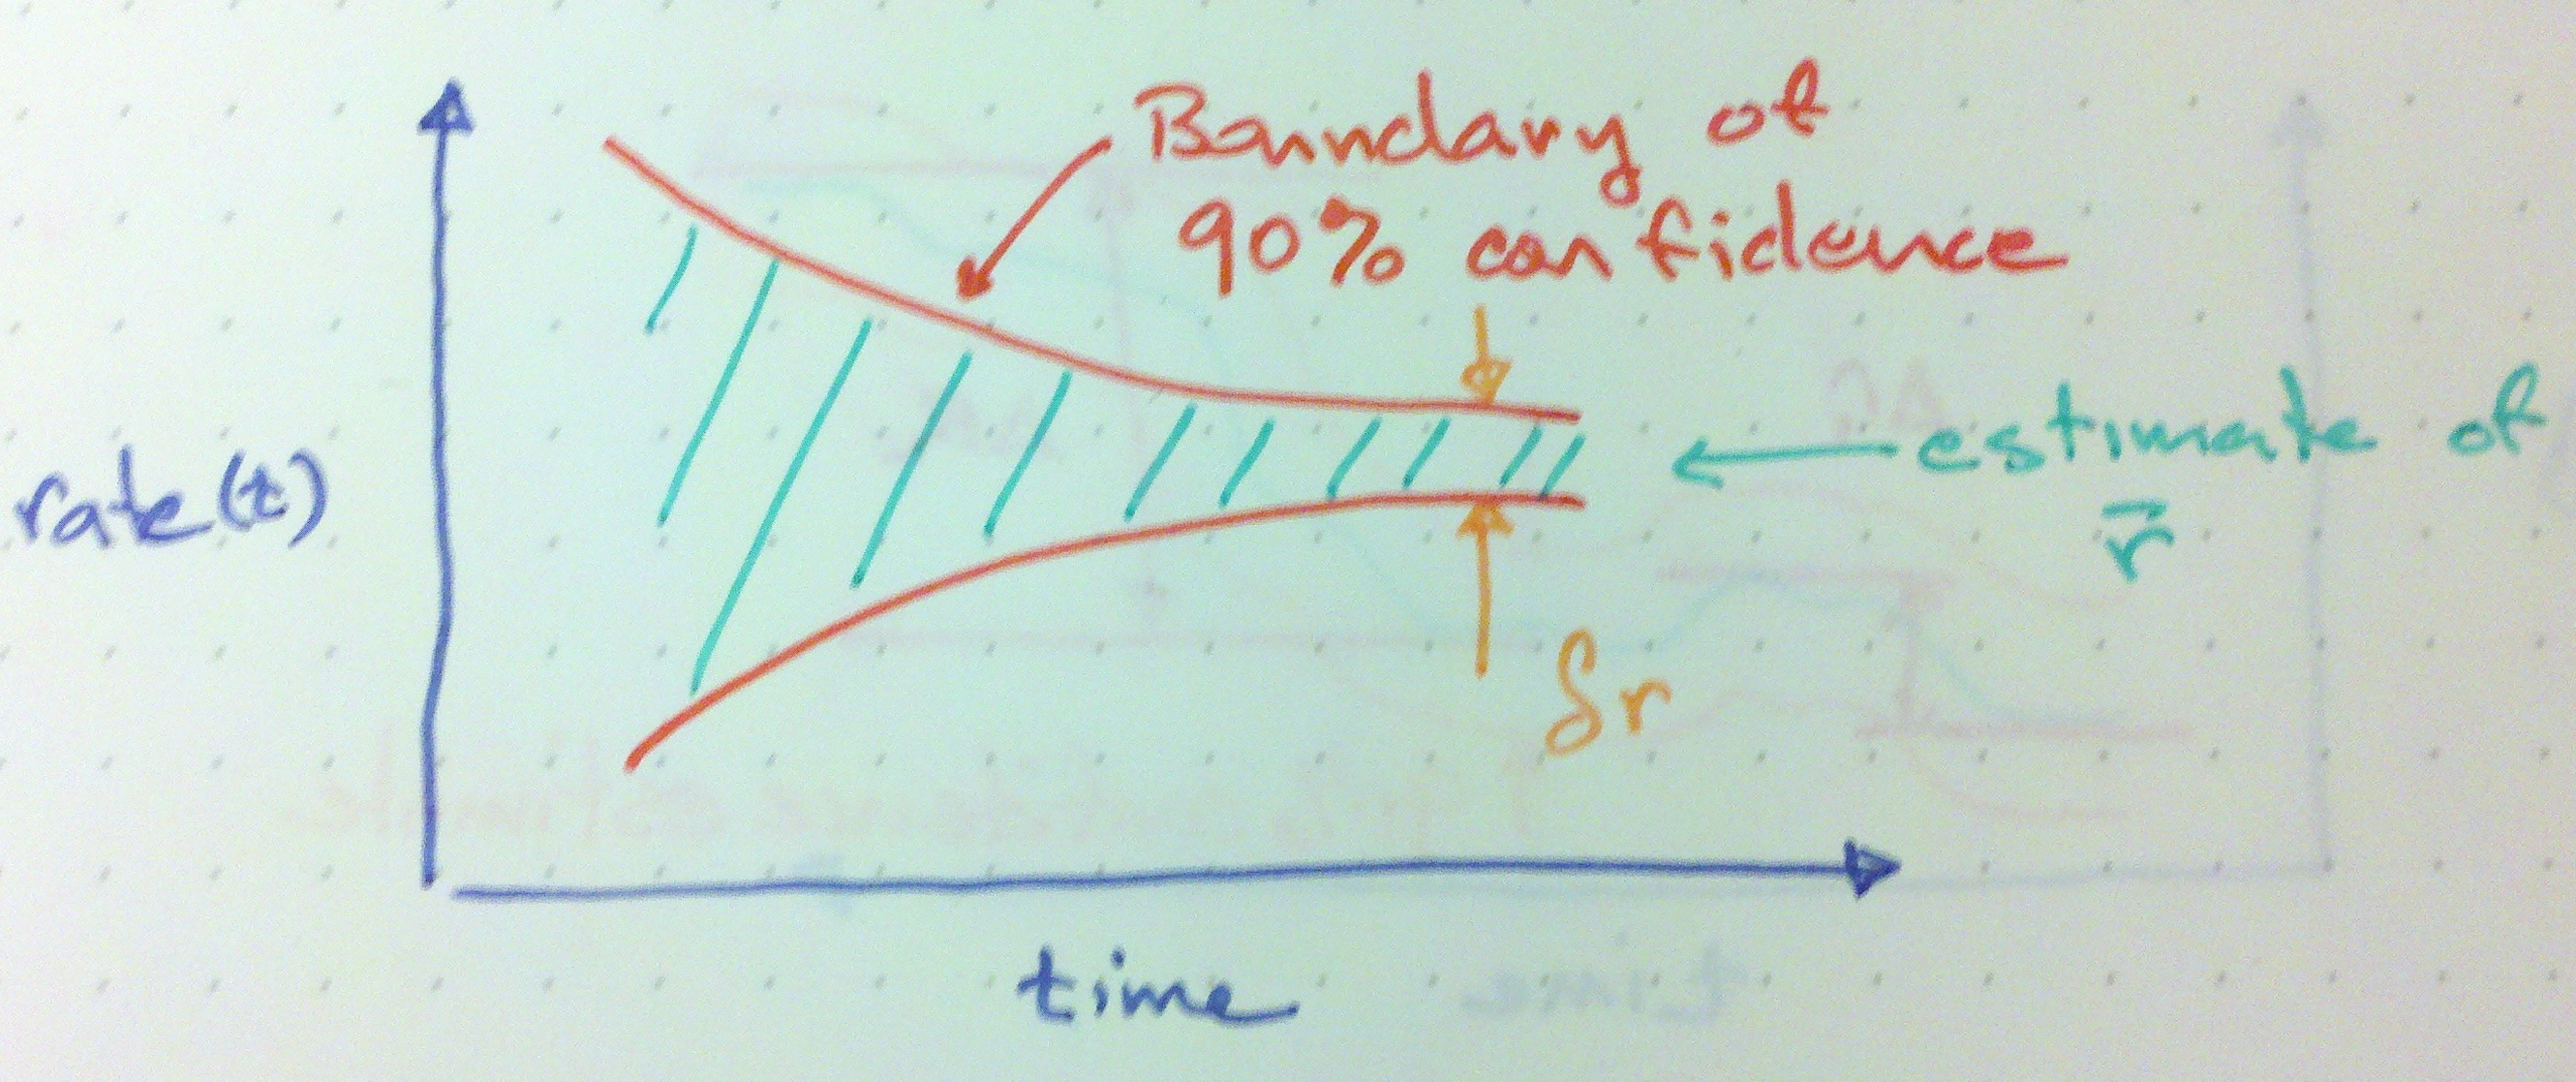
\includegraphics[width=4.0in]{./imgs/confidence.jpg}
	\end{center}
	\caption{Uncertainty in the estimated rate of activities goes down as we observe more events. }
    	\label{fig:confidence}
\end{figure}
%
%
%%%%%


%%%%%
% figure
%
\begin{figure}[h]
    \centering
    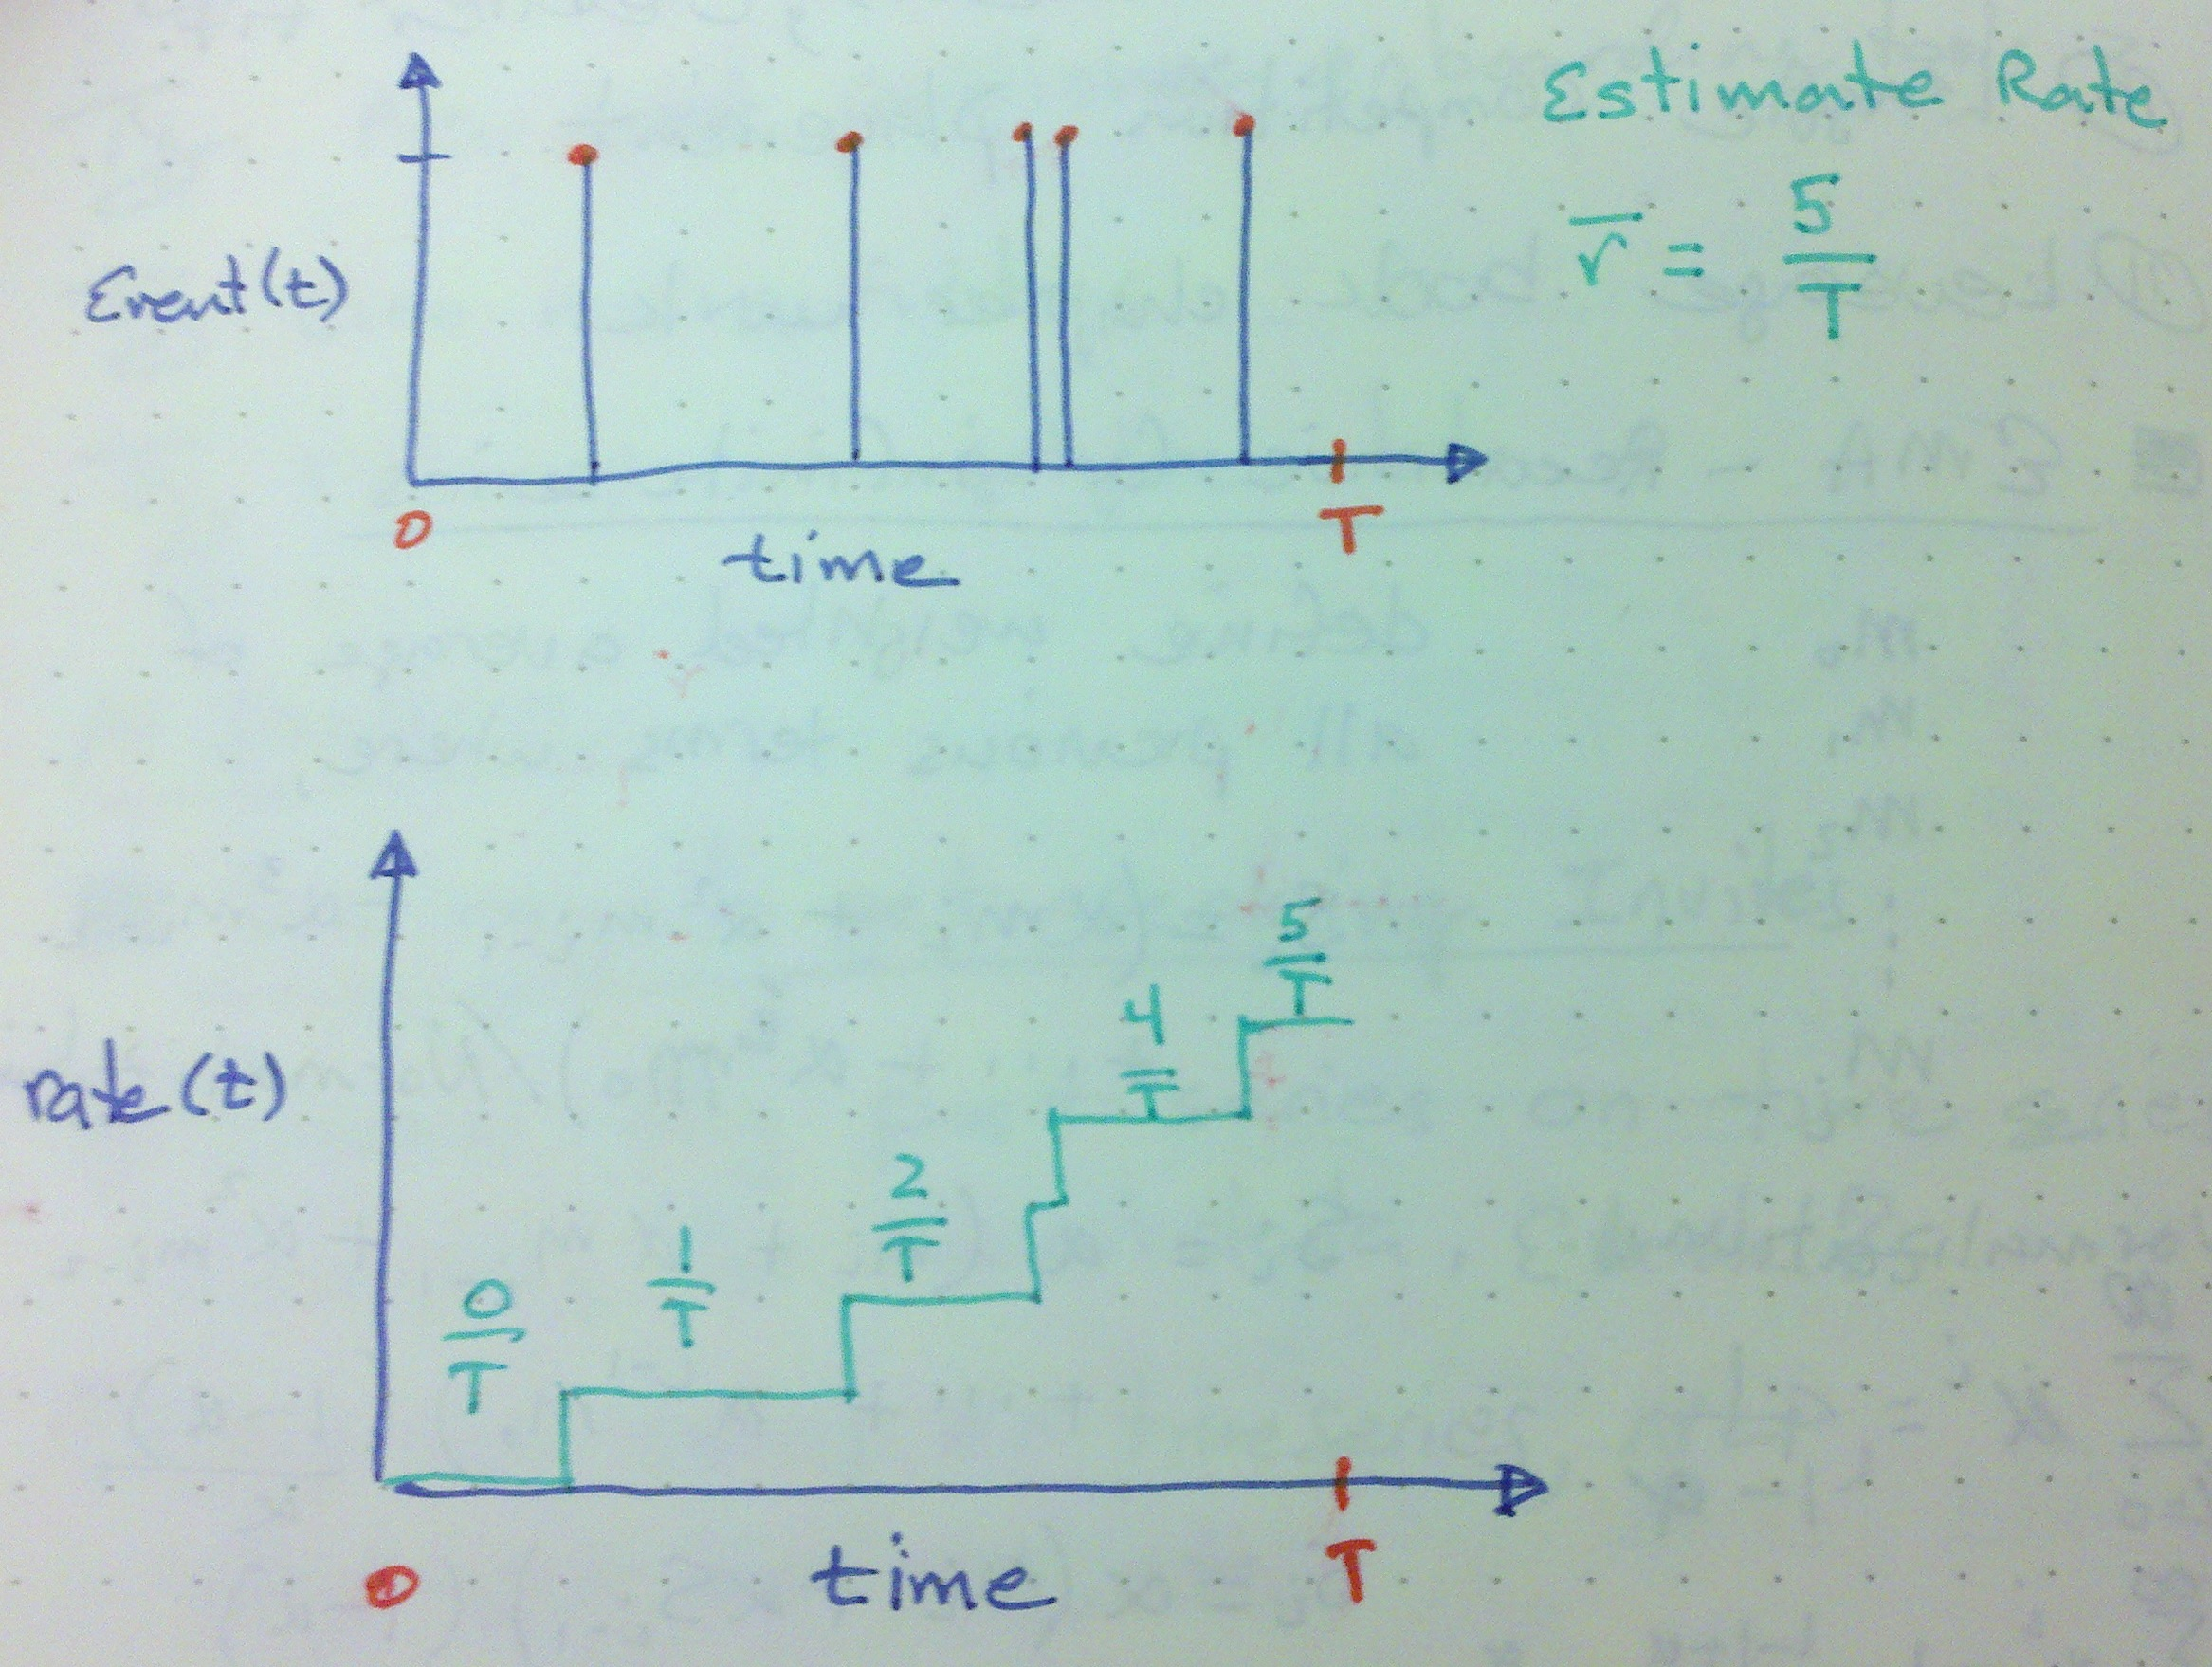
\includegraphics[width=4.0in]{./imgs/events.jpg}
    \caption{Events and rate estimates}
    \label{fig:events}
\end{figure}
%
%
%%%%%



We need to define ``signal'' in a way that provides for tractable calculation.  There is a trade off between our confidence in the estimated activity rate magnitude of the change in  activity rate.  If our estimate of activity rate is very uncertain, large variations are merely expected variations for infrequent events.  Conversely, if your confidence in our estimate of activity rate is high (say, better than 95\%, for example) then we can detect small changes in activity rate.  We say we observe a valid signal in a time series when the activity rate has changed by more than the sensitivity $\Delta r$.  That is,

\begin{equation}
    \label{eq:signal}
    | r(t_f) - r(t_i) | \geq \Delta r
\end{equation}

The time scale of the change, $T_l = t_f - t_i$, is the Signal Latency.  This definition implies that the we must observe activities for a time $T > T_l$ to observe the signal, $\Delta r$.

%%%%%%%%%%%%%%%%%%%%%%%%%%%%%%%%%%
\subsection{Signal-Confidence Criteria} 

We will be estimating the activity rate by Eq. \ref{eq:rateEst} by counting activities for a pre-determined time.  The number of counts in any given period (sample) will be distributed about the true mean of the distribution. As we count more activities, our estimate of rate will converge to the true value.  If we count thousands of activities per minute, our confidence of the estimate of activity rate will be very high after a short time.  For rare activities, we will have to count for a longer time before we have a high level of confidence in our rate estimate.

Referring to the signal definition Eq. \ref{eq:signal}, we can establish a rough criteria for confidence in terms of signal: 

\begin{equation}
    \label{eq:criteria}
    \delta r << \Delta r.
\end{equation}

The variation of the observed number from the average number will decrease with increasing time or increasing rate (the number of activities counted).

The help quantify this inequality, we introduce a criteria factor $\eta$ that quantifies how much larger the change in rate should be, relative to the uncertainty in the rate estimate:

\begin{equation}
    \label{eq:criteriaParam}
    \eta \delta r = \Delta r
\end{equation}
where $\eta >> 1$ when the criteria is fulfilled.

As will be detailed below, the criteria represents trade-offs of number of the number activities (cost of collection and licensing), time (signal latency--how long we have to wait to know the rate has changed), confidence (reliability of estimates of rate), and the size of the rate change we can detect $\Delta r$. These trade offs are summarized in the Table \ref{tab:tradeoff}.


%%%%%
% figure
%
\begin{figure}[h]
    \centering
    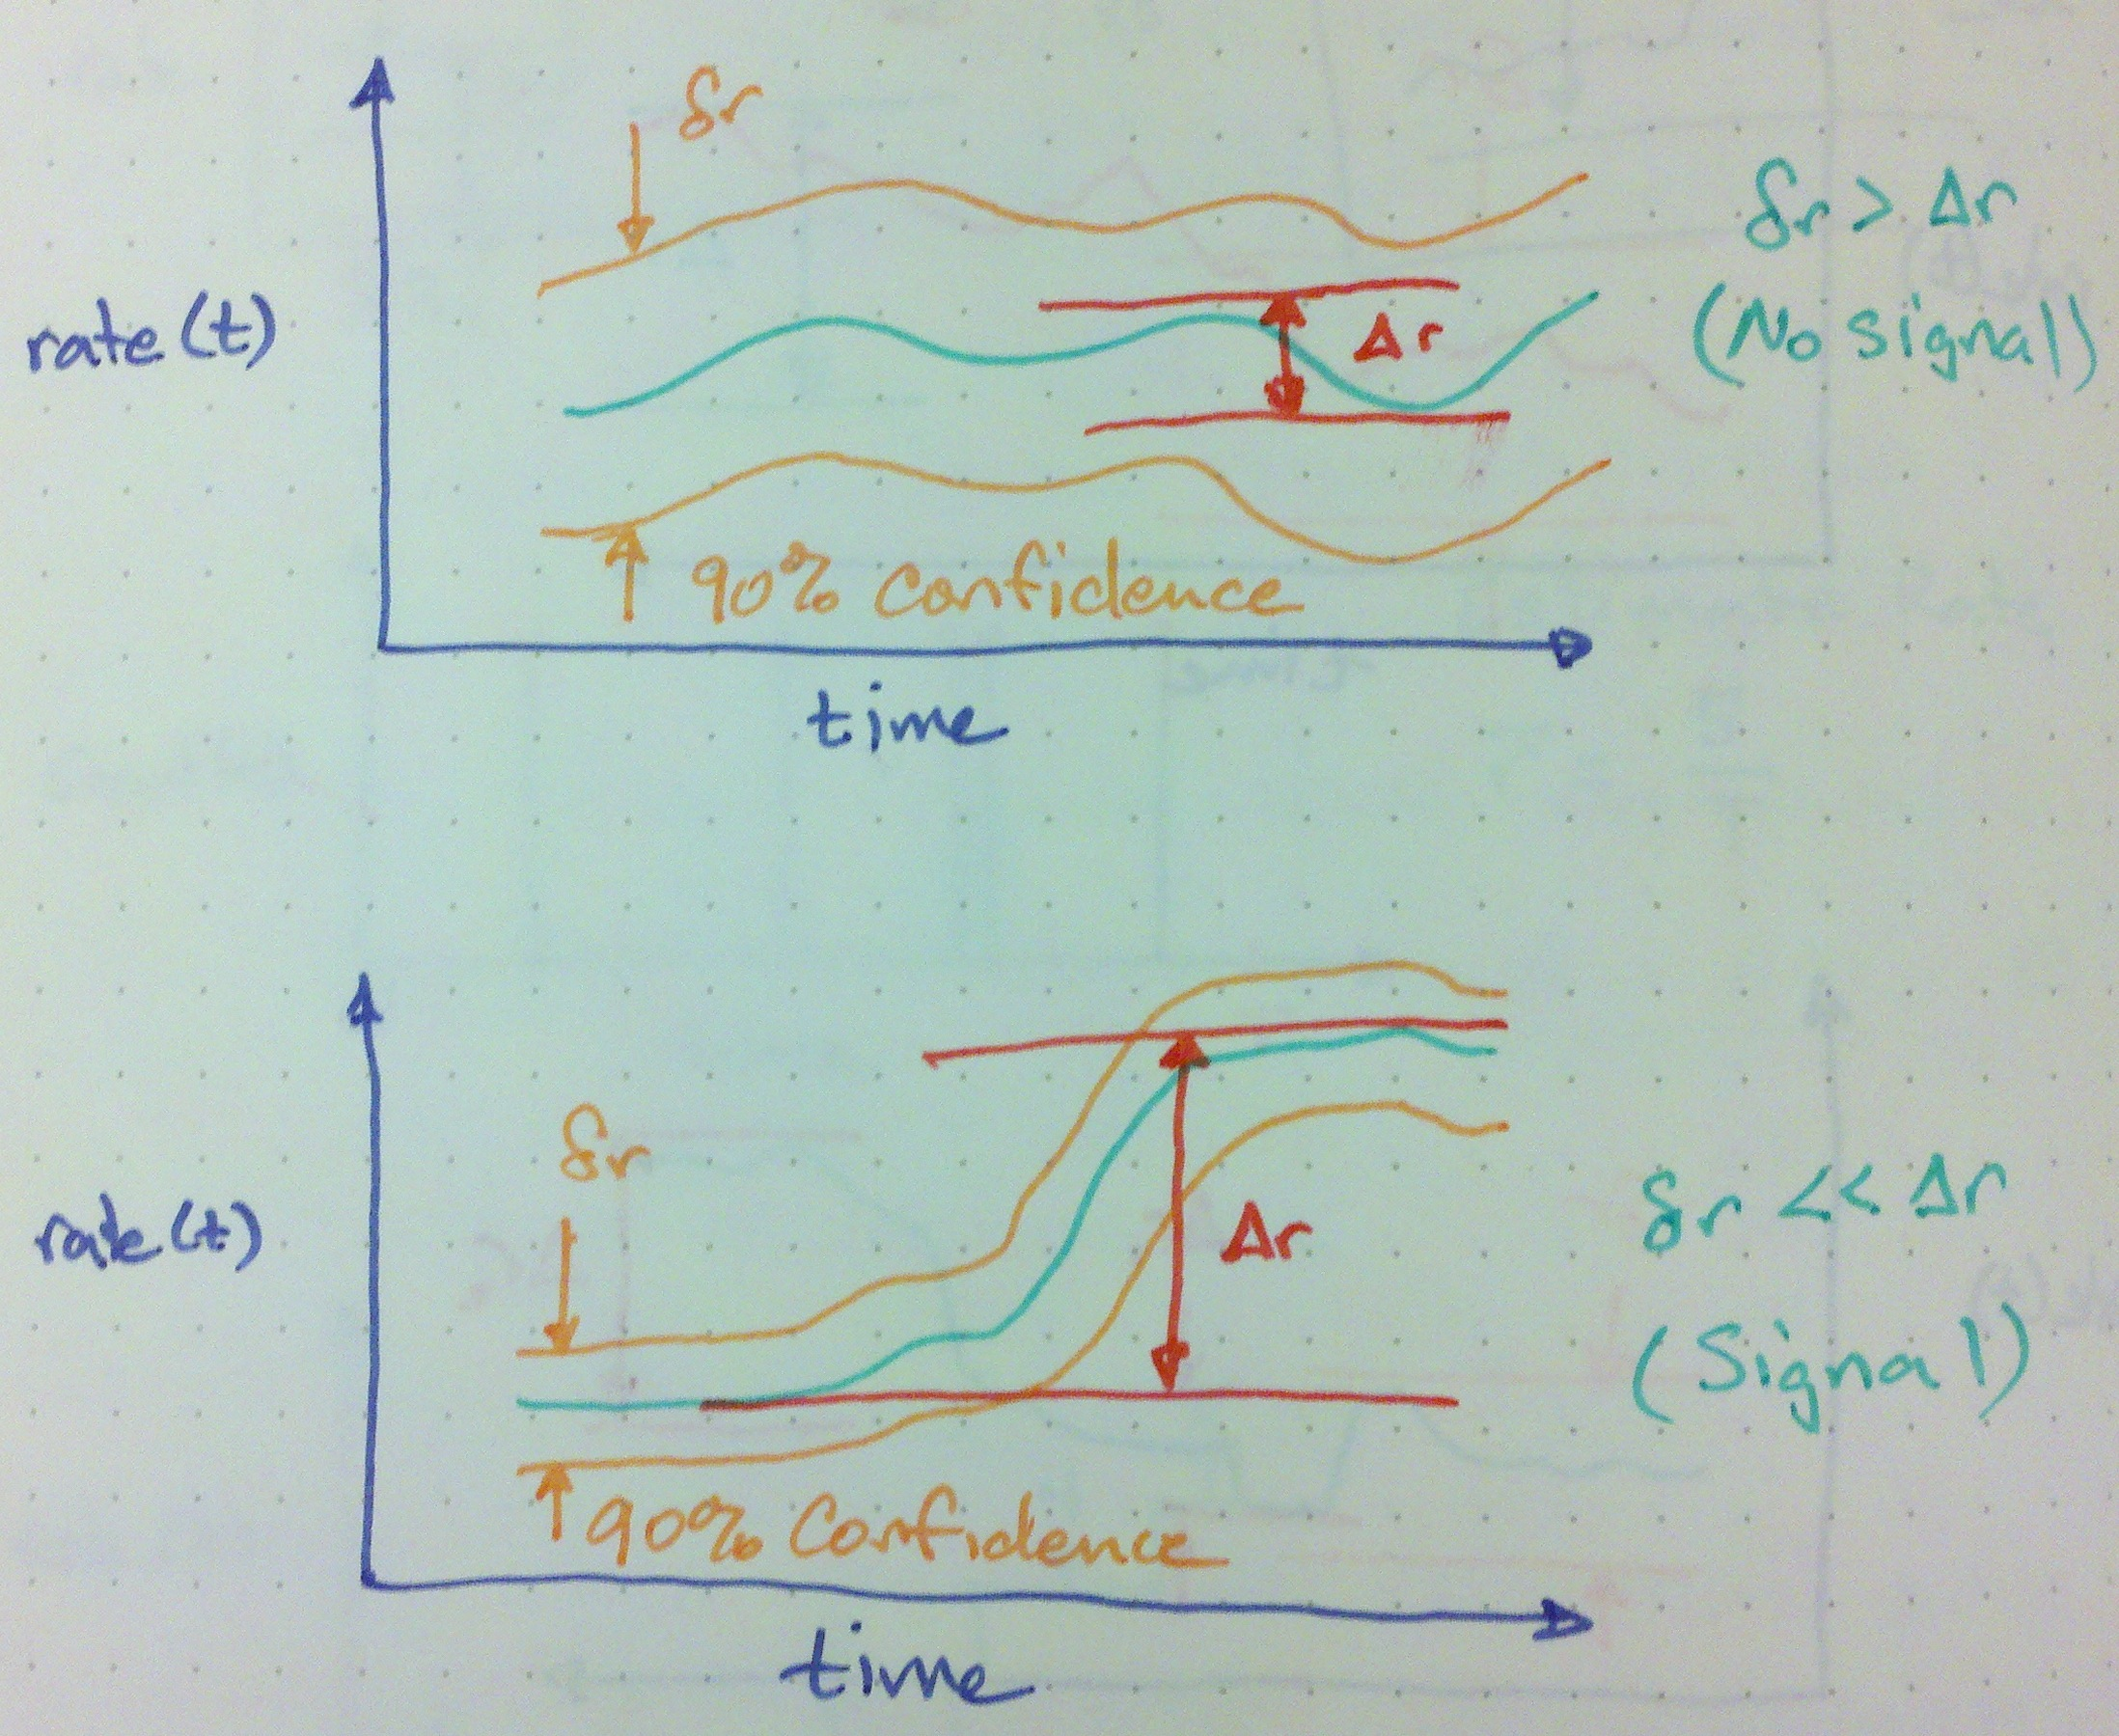
\includegraphics[width=4.0in]{./imgs/signal.jpg}
        \caption{A signal can be detected when the change in rate is greater than the uncertainty in the rate estimates.}
    \label{fig:signal}
\end{figure}
%
%
%%%%%


\begin{table}
\caption{Summary of model trade-offs.}
\label{tab:tradeoff}
    \begin{tabular}{l| m{7cm}}
     \hline
Want to...  & Actions \\
\hline
Minimize Activities Analyzed   & (decrease $N$)  \\
                                  & increase $\Delta r$ (decrease signal sensitivity)  \\
                                  & decrease confidence (E.g. from 95\% to 90\% )  \\
\hline	
Increase Signal sensitivity   & (decrease $\Delta r$)  \\
                                  & increase $T$ (increase number of buckets ($k$)  \\
                                  & or increase bucket size ($\Delta t$) )  \\
                                  & increase activity rate ($r$) by broadening filter or increase PowerTrack sampling \\
\hline
Decrease Signal Latency      & (decrease $T_l$)  \\
                                 & decrease signal sensitivity $\Delta r$  \\
                                 & decrease confidence factor ($\alpha$) \\
                                 & increase activity rate ($r$) by broadening filter or increase PowerTrack sampling \\
\hline
Decrease Signal Uncertainty & (decrease $\delta r$ or increase $\eta$) \\
                          	  & increase $T$ (increase number of buckets ($k$)  \\
                                 & or increase bucket size ($\Delta t$) )  \\
                                 & increase activity counts (increase $N$, $r$) by broadening filter or increase PowerTrack sampling \\
\hline
\end{tabular}

\end{table}


%%%%%%%%%%%%%%%%%%%%%%%%%%%%%%%%%%%%%%%%%%%%%%%%%%%%%%%%%%%%%%%%%%%
\section{Statistics of Time Series of Activities} 


%%%%%%%%%%%%%%%%%%%%%%%%%%%%%%%%%%
\subsection{Time-Between Independent Activities} 

A workable model of counts of rare activities is that the inter-arrival times are exponentially distributed, 

\begin{equation}
    \label{eq:tbe}
    p_{activity}(t) = r e^{-r t}
\end{equation}

This assumption leads a Poission distribution of activity counts over time.

%%%%%%%%%%%%%%%%%%%%%%%%%%%%%%%%%%
\subsection{Poisson Activity Probability} 

The probability of observing $n$ activities in time $t$ when the activity rate is $r$ is given by,
\begin{equation}
    \label{eq:poisson}
    P(n) = \frac{e^{-r t} (r t)^n}{n!}
\end{equation}

The expected value is $E[n]=n=rt$. The mean and variance of the Poisson distribution are both equal to $r$.

%%%%%%%%%%%%%%%%%%%%%%%%%%%%%%%%%%
\subsection{Poisson Confidence Intervals} 

We are counting activities in a defined time interval to estimate the activity rate $r$.  Confidence in the estimate of $r$ goes up as we count more and more activities. Confidence intervals for the Poisson distribution with confidence level $1-\alpha$ are given by

\begin{equation}
    \label{eq:chisqconf}
    \frac{1}{2T} \chi^2(\alpha/2;2n) \leq r \leq \frac{1}{2T} \chi^2(1-\alpha/2;2n+2)
\end{equation}
where $\chi^2$ is the inverse cumulative distribution function, $CDF^{-1}(p; n)$, of the $\chi^2$ distribution.\footnote{A useful approximation to the exact interval is given by  $[ n(1 - \frac{1}{9n} - \frac{z_{\alpha}}{3\sqrt{n}})^3 , (n+1)(1- \frac{1}{9(n+1)} + \frac{z_{\alpha}}{3\sqrt{n+1}})^3]$. }
Note that with this definition of $\alpha$, a confidence interval of 90\% corresponds to $\alpha=0.1$.

% Make the connection between n and N more explicit here

To determine the parameters of our data collection system, we find the value of $n$ for which the time interval and confidence level match our requirements.  Given a set of sensitivity, latency, etc. requirements, we can use the confidence interval to calculate any one of the parameters. 

Calculations for various design choices and an unknown are illustrated in the next section.  First, let's look at some useful limits and approximations for calculating confidence intervals.

%%%%%%%%%%%%%%%%%%%%%%%%%%%%%%%%%%
\subsection{Less-Rare Activities} 

For large $n$, the normal approximation makes the interval calculation simpler. When we observe large values of n, the confidence interval can be estimated using the Normal approximation. For example, for $95\%$ confidence interval the interval is symmetric about the mean and given by,

\begin{equation}
    \label{eq:largenconf}
    \bar{r} - 1.95 \sqrt{\bar{r}/n} \leq \hat{r} \leq \bar{r} + 1.95 \sqrt{\bar{r}/n}
\end{equation}

Confidence intervals for activity counts are shown in Table \ref{tab:conf}.

%SUGGESTION: Remove the intervals of approximation, add a column of interval/N to show the narrowing of the C.I. as N increases.
%\begin{table}
%    \begin{tabular}{r|c|c|c|c}
%     \hline
%$N$ & Bounds  & Interval & Bounds & Interval \\ 
% & ($N>>1$) &  ($N>>1$) &  &  \\ 
%\hline 
%1 & - & - & [ 0.0513, 4.743 ] & 4.692\\ 
%2 & - & - & [ 0.3554, 6.295 ] & 5.940\\ 
%3 & - & - & [ 0.8177, 7.753 ] & 6.936\\ 
%4 & - & - & [ 1.366, 9.153 ] & 7.787\\ 
%5 & - & - & [ 1.970, 10.51 ] & 8.542\\ 
%6 & - & - & [ 2.613, 11.84 ] & 9.229\\ 
%7 & - & - & [ 3.285, 13.14 ] & 9.862\\ 
%8 & - & - & [ 3.980, 14.43 ] & 10.45\\ 
%9 & - & - & [ 4.695, 15.70 ] & 11.01\\ 
%10 & - & - & [ 5.425, 16.96 ] & 11.53\\ 
%20 & - & - & [ 13.25, 29.06 ] & 15.80\\ 
%30 & [ 20.99, 39.00 ] & 18.01 & [ 21.59, 40.69 ] & 19.09\\ 
%40 & [ 29.59, 50.40 ] & 20.80 & [ 30.19, 52.06 ] & 21.87\\ 
%50 & [ 38.36, 61.63 ] & 23.26 & [ 38.96, 63.28 ] & 24.32\\ 
%60 & [ 47.25, 72.74 ] & 25.48 & [ 47.85, 74.38 ] & 26.53\\ 
%70 & [ 56.23, 83.76 ] & 27.52 & [ 56.82, 85.40 ] & 28.57\\ 
%80 & [ 65.28, 94.71 ] & 29.42 & [ 65.87, 96.35 ] & 30.47\\ 
%90 & [ 74.39, 105.6 ] & 31.20 & [ 74.98, 107.2 ] & 32.25\\ 
%100 & [ 83.55, 116.4 ] & 32.89 & [ 84.13, 118.0 ] & 33.94\\ 
%200 & [ 176.7, 223.2 ] & 46.52 & [ 177.3, 224.8 ] & 47.55\\ 
%300 & [ 271.5, 328.4 ] & 56.97 & [ 272.0, 330.0 ] & 58.00\\ 
%400 & [ 367.1, 432.8 ] & 65.79 & [ 367.6, 434.4 ] & 66.81\\ 
%500 & [ 463.2, 536.7 ] & 73.56 & [ 463.7, 538.3 ] & 74.57\\ 
%750 & [ 704.9, 795.0 ] & 90.09 & [ 705.5, 796.6 ] & 91.10\\ 
%1000 & [ 947.9, 1052. ] & 104.0 & [ 948.5, 1053. ] & 105.0\\ 
%\hline
%\end{tabular}
%\caption{Confidence intervals for number of counts in time $T$.  Rate confidence range is $\delta N/T$.  The large $N$ approximation is shown when the boundaries of within 5\% of the exact value.}
%\label{tab:conf}
%\end{table}

\begin{table}
    \begin{tabular}{r|c|c|c|c|c}
     \hline
N & Bounds (N>>1) & Interval (N>>1) & Bounds & Interval & Relative Interval\\ 
\hline 
1 & - & - & [0.0513, 4.7439] & 4.6926 & 4.6926\\ 
2 & - & - & [0.3554, 6.2958] & 5.9404 & 2.9702\\ 
3 & - & - & [0.8177, 7.7537] & 6.9360 & 2.3120\\ 
4 & - & - & [1.3663, 9.1535] & 7.7872 & 1.9468\\ 
5 & - & - & [1.9701, 10.5130] & 8.5429 & 1.7086\\ 
6 & - & - & [2.6130, 11.8424] & 9.2294 & 1.5382\\ 
7 & - & - & [3.2853, 13.1481] & 9.8628 & 1.4090\\ 
8 & - & - & [3.9808, 14.4346] & 10.4538 & 1.3067\\ 
9 & - & - & [4.6952, 15.7052] & 11.0100 & 1.2233\\ 
10 & - & - & [5.4254, 16.9622] & 11.5368 & 1.1537\\ 
20 & - & - & [13.2547, 29.0620] & 15.8074 & 0.7904\\ 
30 & [20.9908, 39.0092] & 18.0185 & [21.5940, 40.6905] & 19.0965 & 0.6366\\ 
40 & [29.5970, 50.4030] & 20.8059 & [30.1957, 52.0694] & 21.8736 & 0.5468\\ 
50 & [38.3691, 61.6309] & 23.2617 & [38.9647, 63.2871] & 24.3223 & 0.4864\\ 
60 & [47.2590, 72.7410] & 25.4820 & [47.8523, 74.3896] & 26.5373 & 0.4423\\ 
70 & [56.2382, 83.7618] & 27.5237 & [56.8297, 85.4046] & 28.5749 & 0.4082\\ 
80 & [65.2880, 94.7120] & 29.4240 & [65.8780, 96.3500] & 30.4720 & 0.3809\\ 
90 & [74.3955, 105.6045] & 31.2089 & [74.9844, 107.2385] & 32.2541 & 0.3584\\ 
100 & [83.5515, 116.4485] & 32.8971 & [84.1393, 118.0793] & 33.9400 & 0.3394\\ 
200 & [176.7383, 223.2617] & 46.5235 & [177.3205, 224.8744] & 47.5539 & 0.2378\\ 
300 & [271.5103, 328.4897] & 56.9794 & [272.0900, 330.0942] & 58.0042 & 0.1933\\ 
400 & [367.1029, 432.8971] & 65.7941 & [367.6812, 434.4968] & 66.8156 & 0.1670\\ 
500 & [463.2200, 536.7800] & 73.5601 & [463.7972, 538.3765] & 74.5793 & 0.1492\\ 
750 & [704.9538, 795.0462] & 90.0923 & [705.5295, 796.6375] & 91.1080 & 0.1215\\ 
1000 & [947.9852, 1052.0148] & 104.0297 & [948.5598, 1053.6031] & 105.0433 & 0.1050\\ 
\end{tabular}
\caption{Confidence intervals for number of counts in time $T$.  Rate confidence range is $\delta N/T$.  The large $N$ approximation is shown when the boundaries of within 5\% of the exact value.}
\label{tab:conf}
\end{table}
% \delta N (table caption) should be defined somewhere.

%%%%%%%%%%%%%%%%%%%%%%%%%%%%%%%%%%
\subsection{Confidence Intervals on Bucketed Time series}

For many reasons, counts may be collected in buckets of some pre-defined time length.  The rate information may by more naturally calculated by bucket rather than the total time $T$ required by our confidence requirements. In general, define the relationship between $T$ and the bucket size (constant) as,

\begin{equation}
    \label{eq:bucket}
    \Delta t = \frac{T}{k}
\end{equation}
where $k$ is the number of buckets that we need to aggregate to observe for time $T$. This parameter can be used to calculate a corresponding signal latency, $k_l = T_l/\Delta t$.

Resolution times are interchangeable with number of buckets $k$ given $\Delta t << T$.  In general, the
bucket resolution time will not be an even multiple of the bucket size.  In this case, imposing the calculation of average rate per bucket $\bar{r} = n/\Delta t$ adds another layer of variability.

See example calculations below for a lookup table of factors.

%%%%%%%%%%%%%%%%%%%%%%%%%%%%%%%%%%
\subsection{Note on Social Media Pulse} 

In the case where something happens in the real world that many social media users can observe and react to (e.g. an earthquake or a celebrity baby photo link leaked on Twitter). The time series of activities will no longer fulfill independence and constant-rate requirements. In these cases, activities can be characterized by the mathematics of the Social Media Pulse (link!).

These activities are likely to be associated with the change in rate, $\Delta r$, that is the signal we are looking for in the stream.

%%%%%%%%%%%%%%%%%%%%%%%%%%%%%%%%%%
\subsection{Model and Parameters} 

Table \ref{tab:summary} summarizes the parameters of the model.

\begin{table}
    \begin{tabular}{c| m{7cm}}
     \hline
Parameter  & Definition \\
\hline	
$N$ & Number of activities in time $T$\\
$T$ & Observation time\\
$\Delta t$ & Bucket size (for bucketed data where $\Delta t <T$) \\
$k$ & Observation time measured in buckets ($k=T/\Delta t$) \\
$r$ & Activity rate \\
$\bar{r} = N/T$ & Estimate of activity rate \\
$\delta r$ & Uncertainty of rate estimate \\
$\alpha$ & Confidence fraction of rate estimate range\\
$\Delta r$ & Change in activity rate that defines signal \\
$T_l$ & Signal latency \\
$\eta$ & Rate signal criteria factor \\
\hline
\end{tabular}
\caption{Summary of model parameters.}
\label{tab:summary}
\end{table}

%%%%%%%%%%%%%%%%%%%%%%%%%%%%%%%%%%%%%%%%%%%%%%%%%%%%%%%%%%%%%%%%%%%
\section{Example Calculations} 

We present some example calculation to make this concrete and illustrate the use of the lookup tables.

%%%%%%%%%%%%%%%%%%%%%%%%%%%%%%%%%%
\subsection{Estimate the Optimal PowerTrack Sampling Operator Value} 

To do \ldots

%%%%%%%%%%%%%%%%%%%%%%%%%%%%%%%%%%
\subsection{Estimate Signal Latency} 

% first pass at calc, 2013-04-18, BL

How long does it take to identify a change in the activity rate as a signal?

As an example for calculating $T_{l}$, we choose a specific signal $\Delta r = \frac{10}{T}$.  The time $T_{l}$ that it takes to observe this signal $\Delta r$, or equivalently, the number of buckets, $k$, depends the total number of activities $N_t$ that we must observe to have a credible estimate of the activity rate. Because activities are infrequent, we will look up the confidence interval for small numbers of activities this up in Table \ref{tab:conf}.  As $N_t$ increases, the $90\%$ confidence interval length $I$ narrows around the average rate $\delta r$ decreases.  See Equation \ref{...}3??.  We need to find the value for $N$ at which point $\delta r$ has decreased enough to allow us to see our signal $\Delta r = \frac{10}{T}$.  

Choosing $\eta=1$, we see in Table \ref{tab:conf} that for $\Delta r = \frac{10}{T}$, we must have $N\geq7$ causing $I > 10\eta$ in order to observe our signal.  Notice that $N_t=7$ is the point after which we could first observe a signal.  Thus, we say that $T_{l}>T_{N_t}$ defines the time that it takes to observe a signal, which means that signal latency is greater than the amount of time that it takes to collect $N_t$ activities.  Takes 2 periods to get the calculation> have to calculate the rate in the first then the second and compare.

We can decrease $T_{l}$ in several ways.  First, we could try improving the rate at which we achieve $N_t$ by  increasing our PowerTrack sampling.  Otherwise, we could decrease $T_{l}$ as we narrow $I$ through a lower confidence level $(1-\alpha)$.  The lower confidence level tightens $I$ around smaller $N$ allowing the potential signal to become clearer faster, but this goal is accomplished at the cost of decreased confidence.  Another basic option is to simply choose a smaller (larger?) signal size such as $\Delta r = \frac{5}{T}$ from our previous example.  All of these strategies would decrease $T_{l}$.



%%%%%%%%%%%%%%%%%%%%%%%%%%%%%%%%%%
\subsection{Estimate Signal Resolution}
% first pass at calc, 2013-03-12, JM

Suppose we would like to determine the magnitude of a signal change needed to 
classify it as significant. As shown in Equation~\ref{eq:criteriaParam}, 
classifying a signal $\Delta r$ as significant depends on the choice of criteria factor 
$\eta$ and the observation parameters that determine the uncertainty $\delta r$. 
Specifically, we will need to choose a criteria factor $\eta$ and confidence levexl 
$1-\alpha$, and our observation will be characterized by total activity counts $N$ 
and total time $T$.

%Based on the Poisson confidence intervals in Equation~\ref{eq:chisqconf}, our 
%significant signal must then either be 
%
%\begin{equation}
%	\label{eq:sigSig1}
%\Delta r - \bar{r} > \frac{1}{2} \chi^2(1-\alpha/2;2N+2), 
%\end{equation}
%or lower than 
%
%\begin{equation}
%	\label{eq:sigSig2}
%\bar{r} - \Delta r < \frac{1}{2} \chi^2(\alpha/2;2N). 
%\end{equation}


Let us assume we have decided to classify as significant a signal with $\eta$ = 10, or 
$\Delta r > 10\delta r$. Furthermore, we have chosen a 90\% confidence interval 
($\alpha = 0.1$), and observed $N$=10,000 activities over a period of $T$=1 minute 
(60 seconds) for an estimated activity rate of $\bar r = 167~\si{\per\second}$. We next use 
Equation~\ref{eq:chisqconf} to calculate the interval of activities for our 
90\% confidence level, and divide by observation period $T$ to obtain the corresponding 
minimum significant activity rate $\delta r = 5~\si{\per\second}$. Recall, however, 
that we have also specified a criteria factor $\eta = 10$. Therefore, in this example, 
in order to classify the change in rate as significant, we must observe a change at the 
level of 
$\Delta r = \eta \delta r = 10 (5~\si{\per\second}) = 50~\si{\per\second}$. 
For an increasing activity rate, this corresponds to a total activity rate of 
$167~\si{\per\second} + 50~\si{\per\second} = 217~\si{\per\second}$. For a decreasing 
rate, $117~\si{\per\second}$.

% how much to worry that confidence went down for smaller rate final rate


% Procedure for this calculation:
% 	Using the tables.py script, calculate poisson_bounds1() for N=10000, confidence=0.90, 
% 	and the resulting bounds (to one decimal) are [9836.1, 10166.1]. This is an interval of count 
%	of activities; the corresponding bounds on the rate are given by this interval divided by 
% 	the time period, T=60 s: (10166.1-9836.1)/60 ~ 5 /s. 



%%%%%%%%%%%%%%%%%%%%%%%%%%%%%%%%%%%%%%%%%%%%%%%%%%%%%%%%%%%%%%%%%%%
\section{Conclusion and References} 

This is intended to help you use the Gnip social data streams more effectively.  If you find errors or have comments, please email shendrickson@gnip.com. Thank you.

%\section{Lookup Table}
%
%%% Table generated by formatTable utility %%
%%% add \usepackage[group-separator={,}]{siunitx}
%%%
%\begin{table}
%\begin{tabular}{|S|S|S|S|}
%\hline
%{Counts/Bucket} & { Buckets} & { Confidence} & { $\Delta Count$} \\
%\hline
%      1     &    10   &     91.31     &        0.472 7    \\
%      1     &    20   &     90.85     &        0.349 6    \\
%      1     &    30   &     89.73     &        0.290 3    \\
%      1     &    40   &     90.32     &        0.253 2    \\
%      1     &    50   &     90.06     &        0.223 4    \\
%      1     &    60   &     89.74     &        0.207 7    \\
%      1     &    70   &     89.58     &        0.190 1    \\
%      1     &    80   &     89.77     &        0.178 0    \\
%      1     &    90   &     90.02     &        0.170 3    \\
%      2     &    10   &     88.34     &        0.636 4    \\
%      2     &    20   &     88.42     &        0.476 2    \\
%      2     &    30   &     90.24     &        0.419 4    \\
%      2     &    40   &     89.65     &        0.361 5    \\
%      2     &    50   &     90.31     &        0.323 5    \\
%      2     &    60   &     89.76     &        0.295 1    \\
%      2     &    70   &     90.25     &        0.281 7    \\
%      2     &    80   &     90.48     &        0.259 3    \\
%      2     &    90   &     90.01     &        0.241 8    \\
%      3     &    10   &     89.20     &        0.818 2    \\
%      3     &    20   &     90.80     &        0.603 9    \\
%      3     &    30   &     90.16     &        0.500 0    \\
%      3     &    40   &     89.45     &        0.439 0    \\
%      3     &    50   &     90.23     &        0.392 2    \\
%      3     &    60   &     90.23     &        0.357 6    \\
%      3     &    70   &     90.33     &        0.338 0    \\
%      3     &    80   &     89.98     &        0.312 8    \\
%      3     &    90   &     89.79     &        0.296 7    \\
%      4     &    10   &     89.77     &        0.954 5    \\
%      4     &    20   &     90.58     &        0.714 3    \\
%      4     &    30   &     89.93     &        0.580 6    \\
%      4     &    40   &     89.67     &        0.500 0    \\
%      4     &    50   &     89.87     &        0.451 0    \\
%      4     &    60   &     89.89     &        0.418 0    \\
%      4     &    70   &     89.68     &        0.387 3    \\
%      4     &    80   &     90.03     &        0.358 0    \\
%      4     &    90   &     89.77     &        0.340 7    \\
%      5     &    10   &     88.95     &        1.045      \\
%      5     &    20   &     89.51     &        0.785 7    \\
%      5     &    30   &     89.32     &        0.645 2    \\
%      5     &    40   &     90.11     &        0.573 2    \\
%      5     &    50   &     90.31     &        0.509 8    \\
%      5     &    60   &     90.18     &        0.467 2    \\
%      5     &    70   &     90.32     &        0.443 7    \\
%      5     &    80   &     90.15     &        0.407 4    \\
%      5     &    90   &     90.01     &        0.373 6    \\
%\hline
%\end{tabular}
%\end{table}
%%% Table generated by formatTable utility %%
%
%%% Table generated by formatTable utility %%
%%% add \usepackage[group-separator={,}]{siunitx}
%%%
%\begin{table}
%\begin{tabular}{|S|S|S|S|}
%\hline
%{Counts/Bucket} & { Buckets} & { Confidence} & { $\Delta Count$} \\
%\hline
%      6     &    10   &     90.66     &        1.182      \\
%      6     &    20   &     89.91     &        0.857 1    \\
%      6     &    30   &     89.77     &        0.693 5    \\
%      6     &    40   &     90.36     &        0.634 1    \\
%      6     &    50   &     90     &        0.558 8    \\
%      6     &    60   &     89.62     &        0.508 2    \\
%      6     &    70   &     90.28     &        0.485 9    \\
%      6     &    80   &     90.27     &        0.450 6    \\
%      6     &    90   &     89.90     &        0.417 6    \\
%      7     &    10   &     89.49     &        1.227      \\
%      7     &    20   &     89.81     &        0.928 6    \\
%      7     &    30   &     89.71     &        0.758 1    \\
%      7     &    40   &     89.56     &        0.670 7    \\
%      7     &    50   &     90.12     &        0.607 8    \\
%      7     &    60   &     90.04     &        0.549 2    \\
%      7     &    70   &     90.24     &        0.514 1    \\
%      7     &    80   &     89.79     &        0.481 5    \\
%      7     &    90   &     89.97     &        0.450 5    \\
%      8     &    10   &     90.57     &        1.364      \\
%      8     &    20   &     89.52     &        0.976 2    \\
%      8     &    30   &     89.82     &        0.806 5    \\
%      8     &    40   &     90.09     &        0.719 5    \\
%      8     &    50   &     90.28     &        0.647 1    \\
%      8     &    60   &     89.95     &        0.590 2    \\
%      8     &    70   &     89.94     &        0.549 3    \\
%      8     &    80   &     89.86     &        0.512 3    \\
%      8     &    90   &     89.80     &        0.478 0    \\
%      9     &    10   &     89.57     &        1.409      \\
%      9     &    20   &     89.86     &        1.048      \\
%      9     &    30   &     89.77     &        0.871 0    \\
%      9     &    40   &     89.88     &        0.768 3    \\
%      9     &    50   &     89.61     &        0.676 5    \\
%      9     &    60   &     90.03     &        0.631 1    \\
%      9     &    70   &     89.97     &        0.584 5    \\
%      9     &    80   &     90.10     &        0.555 6    \\
%      9     &    90   &     90.01     &        0.511 0    \\
%     10      &    10   &     89.87     &        1.500      \\
%     10      &    20   &     89.37     &        1.095      \\
%     10      &    30   &     89.93     &        0.919 4    \\
%     10      &    40   &     90.10     &        0.792 7    \\
%     10      &    50   &     89.70     &        0.715 7    \\
%     10      &    60   &     89.66     &        0.655 7    \\
%     10      &    70   &     89.98     &        0.612 7    \\
%     10      &    80   &     89.89     &        0.574 1    \\
%     10      &    90   &     90.12     &        0.544 0    \\
%     11      &    10   &     90.46     &        1.591      \\
%\hline
%\end{tabular}
%\end{table}
%%% Table generated by formatTable utility %%
%
%%% Table generated by formatTable utility %%
%%% add \usepackage[group-separator={,}]{siunitx}
%%%
%\begin{table}
%\begin{tabular}{|S|S|S|S|}
%\hline
%{Counts/Bucket} & { Buckets} & { Confidence} & { $\Delta Count$} \\
%\hline
%     11      &    20   &     90.16     &        1.167      \\
%     11      &    30   &     90.28     &        0.951 6    \\
%     11      &    40   &     89.96     &        0.841 5    \\
%     11      &    50   &     89.94     &        0.764 7    \\
%     11      &    60   &     90.12     &        0.696 7    \\
%     11      &    70   &     89.77     &        0.633 8    \\
%     11      &    80   &     89.94     &        0.598 8    \\
%     11      &    90   &     90.17     &        0.571 4    \\
%     12      &    10   &     90.43     &        1.636      \\
%     12      &    20   &     89.30     &        1.190      \\
%     12      &    30   &     90.21     &        1      \\
%     12      &    40   &     90.10     &        0.890 2    \\
%     12      &    50   &     90.17     &        0.803 9    \\
%     12      &    60   &     90.15     &        0.729 5    \\
%     12      &    70   &     89.88     &        0.676 1    \\
%     12      &    80   &     90.11     &        0.629 6    \\
%     12      &    90   &     89.80     &        0.598 9    \\
%     13      &    10   &     89.78     &        1.682      \\
%     13      &    20   &     90.14     &        1.286      \\
%     13      &    30   &     90.28     &        1.048      \\
%     13      &    40   &     89.79     &        0.914 6    \\
%     13      &    50   &     90.07     &        0.833 3    \\
%     13      &    60   &     90.35     &        0.754 1    \\
%     13      &    70   &     89.77     &        0.697 2    \\
%     13      &    80   &     90.16     &        0.654 3    \\
%     13      &    90   &     90.04     &        0.615 4    \\
%     14      &    10   &     90.02     &        1.773      \\
%     14      &    20   &     90.38     &        1.310      \\
%     14      &    30   &     89.69     &        1.097      \\
%     14      &    40   &     89.88     &        0.939 0    \\
%     14      &    50   &     90.06     &        0.862 7    \\
%     14      &    60   &     89.65     &        0.762 3    \\
%     14      &    70   &     90.05     &        0.725 4    \\
%     14      &    80   &     89.97     &        0.691 4    \\
%     14      &    90   &     89.96     &        0.642 9    \\
%     15      &    10   &     90.39     &        1.864      \\
%     15      &    20   &     89.95     &        1.333      \\
%     15      &    30   &     90.05     &        1.129      \\
%     15      &    40   &     90.06     &        0.987 8    \\
%     15      &    50   &     89.75     &        0.872 5    \\
%     15      &    60   &     89.94     &        0.803 3    \\
%     15      &    70   &     90.05     &        0.753 5    \\
%     15      &    80   &     89.97     &        0.697 5    \\
%     15      &    90   &     90.20     &        0.675 8    \\
%     16      &    10   &     90.30     &        1.909      \\
%\hline
%\end{tabular}
%\end{table}
%% Table generated by formatTable utility %%


%%%%%%%

%\subsection{Doubling Period}
%
%The time it takes to double $V$ is noted as $t_{2x}$ and given by,
%\begin{eqnarray*}
%    \label{eq:double-calc}
%     V(t)  = & V_0 \exp ( \alpha t ) \\
%     V(t_{2x})  = & V_0 \exp ( \alpha (t_{2x}) ) \\
%    = & 2 V_0 \exp ( \alpha t ) \\
%    2 = & \exp(\alpha t_{2x} \\
%    \log 2 = & \alpha t_{2x}
%\end{eqnarray*}
%Solving for $t_{2x}$,
%\begin{equation}
%    \label{eq:double}
%    t_{2x} = \frac{\log 2}{\alpha} 
%\end{equation}
%
%\subsection{Apply to some twitter data}

%\begin{figure}
%    \centering
%    \includegraphics[width=4.0in]{stacked_year_fig.png}
%    \caption{Log-Twitter Volume Through 2010}
%    \label{simulationfigure}
%\end{figure}

%The Table shows 4 regions of exponential growth in monthly Twitter volume from its beginnings in 2006 through 2010. The first period ends in April 2007, the second ends in December 2008.  The third period of faster growth is short, lasting only a few months. The last period spans August 2009 through December 2010.
%
%\begin{table}
%    \begin{tabular}{|c|r|l|l|l}
%     \hline
%Month    & Twitter Volume  &       LN(Volume) & Parameters \\
%\hline	
%1&	638&	6.45833& 	$\alpha = 0.61948$ per month \\
%2&	1,918&	7.55903&	 $t_{2x} = 1.11891$	months \\
%3&	2,002&	7.60190& 	85.8\%	growth/month \\
%\ldots & & &		 \\
%14&	2,005,933&	14.5116&		 \\
%\hline
%15&	2,785,237&	14.8398& $\alpha = 	0.1868$ /month \\
%16&	3,016,238&	14.9195& 	$t_{2x} = 3.70976$	months \\
%17&	3,673,111&	15.1165&	 20.5\%	growth/month \\
%\ldots & & &			 \\
%34&	42,517,816&	17.5654&	 \\
%\hline	
%35&	56,861,590&	17.8561&	$\alpha = 0.48043$ /month \\
%36&	72,301,087&	18.0963&	$t_{2x} = 1.44275$	months \\
%37&	117,404,715&	18.5811&	61.7\%	growth/month \\
%\ldots & & &		\\
%41&	358,626,288&	19.6977&		 \\
%\hline
%42&	393,489,407&	19.7905&	$\alpha = 0.11678$ /month \\
%43&	458,444,722&	19.9433&$t_{2x} = 	5.93501$	months \\
%44&	527,824,897&	20.0842&	12.4\%	growth/month \\
%\ldots & & &		 \\
%58&	2,549,581,037&	21.6591&		 \\
%\hline
%\end{tabular}
%\end{table}


\end{document}
